\documentclass[12pt]{report}
\usepackage{amsmath}
\usepackage{graphicx}
\usepackage{hyperref}
\usepackage{geometry}
\usepackage{float}
\geometry{a4paper, margin=1in}
\usepackage{caption}  % For customizing captions
\usepackage{placeins} % For \FloatBarrier

\title{\textbf{Predicting Sales Data for Rossmann Stores}\\
\large Programming in Python for Business and Life Science Analytics}

\author{
    Emin Alp Bıyık \\
    Kento Ohashi \\
    Elif Yılmaz
}
\date{Summer 2024}

\begin{document}

\maketitle

\chapter{Introduction}
Sales forecasting has become a critical component of business strategy, business management, and operational planning over the years, and its importance is increasing day by day. It involves forecasting future sales based on historical data, market trends, and other relevant factors which vary by industry and problem definition. Accurate sales forecasts enable companies to make informed decisions regarding inventory management, budgeting, and resource allocation, thereby increasing overall business efficiency and competitiveness, which make it very vital for every business environment. More complex and accurate prediction models developed with the widespread use of machine learning have created a revolution by replacing the simple statistical approaches used in the past. For the Summer 2024 term of the Programming in Python for Business and Life Science Analytics course, our project team explored a variety of machine learning algorithms including regression models, decision trees, and XGBoost to predict historical sales data for the Rossmann company. By utilizing these models, we aim to determine the most effective approach by comparing models to predict sales in a dynamic market environment.

\chapter{Literature Review}
Traditional methods of sales forecasting have often failed to capture complex patterns and interactions within sales data. The development of advanced machine learning techniques has also influenced this field (Fattah et al. 2018). For this reason, there has been a transition from traditional methods to machine learning in the industry over the years. This change has been particularly beneficial for inventory management and strategy optimization based on sales forecasts which are very important for companies. Academic studies also show that improved forecasting increases profitability by helping retailers reduce inventory and overstock situations (Fildes et al. 2019).

Different models have various advantages but also limitations for sales forecasting. As it is quite simple and effective, linear regression models are widely used. However, adjustments need to be made to work in high-volume and complex data sets (Dinçoğlu and Aygün 2022). Decision trees provide flexibility by splitting data into subsets based on predictive variables and effectively capturing nonlinear relationships. Studies have shown that combining this model with models such as Random Forest and XGBoost improves prediction performance (Kaushal et al. 2023; Sajawal 2022). Neural networks, especially deep learning models, are game changers in this field. These models perform better than other models at identifying complex patterns and trends in sales data. These models have demonstrated high performance in various comparative studies, becoming powerful tools for retail sales forecasting (Zhang 2005; Seaman 2018).

To conclude, machine learning models offer significant advantages for sales forecasting, especially in the retail industry. Each model has its strengths and weaknesses. Therefore, model selection should be made according to the characteristics of the dataset and prediction goals. In this project, we aimed to utilize regression models, decision trees, and XGBoost models to increase sales forecast accuracy and provide valuable information for making strategic business decisions.

\chapter{Dataset and Features}
The Rossmann sales dataset consists of historical sales data for 1115 stores. The \texttt{train.csv} file includes sales data from January 1, 2013, to July 31, 2015, with features such as Store, Sales, Customers, Open, Promo, StateHoliday, SchoolHoliday, and Date. The \texttt{test.csv} file covers the period from August 1, 2015, to September 17, 2015, focusing on future sales predictions. Additionally, the \texttt{store.csv} file provides supplementary information about each store, including StoreType, Assortment, PromoInterval, CompetitionDistance, CompetitionOpenSinceMonth, CompetitionOpenSinceYear, Promo2, Promo2SinceWeek, and Promo2SinceYear. Table 1 shows the details of the columns for \texttt{stores.csv}, \texttt{train.csv}, and \texttt{test.csv} files. These datasets together enable comprehensive sales analysis and forecasting. However, not all stores have data for each feature on each day and some columns have different data types, so a very detailed data preprocessing step has been conducted and explained in the next chapter.

% \documentclass[12pt]{article}
% \usepackage{array}
% \usepackage{geometry}
% \geometry{a4paper, margin=1in}


\begin{table}[h]
    \centering
    \begin{tabular}{|l|c|c|c|p{4cm}|}
        \hline
        \textbf{Column} & \textbf{store.csv} & \textbf{train.csv} & \textbf{test.csv} & \textbf{Details} \\
        \hline
        Store & x & x & x & storeID (1-1115) \\
        \hline
        DayOfWeek &  & x & x & 1-7 (1-Monday, 7-Sunday) \\
        \hline
        Date &  & x & x & year, month, day \\
        \hline
        Sales &  & x &  & Sales amount \\
        \hline
        Customers &  & x &  & Number of customers \\
        \hline
        Open &  & x & x & Whether the store was open \\
        \hline
        Promo &  & x & x & Whether a promo was active \\
        \hline
        StateHoliday &  & x & x & Factor: 0, a, b, c \newline a= Public holiday, b= Easter holiday, c= Christmas, 0= not holiday \\
        \hline
        SchoolHoliday &  & x & x & Binary: 1 \\
        \hline
        StoreType & x &  &  & Factor: a, b, c, d \\
        \hline
        Assortment & x &  &  & Factor: a, b, c \\
        \hline
        CompetitionDistance & x &  &  & Distance to nearest competitor \\
        \hline
        CompetitionOpenSinceMonth & x &  &  & Month the competition opened \\
        \hline
        CompetitionOpenSinceYear & x &  &  & Year the competition opened \\
        \hline
        Promo2 & x &  &  & Continuation of promo \\
        \hline
        Promo2SinceWeek & x &  &  & Week promo2 started \\
        \hline
        Promo2SinceYear & x &  &  & Year promo2 started \\
        \hline
        PromoInterval & x &  &  & Interval of the promo2 \\
        \hline
    \end{tabular}
    \caption{stores.csv, train.csv, and test.csv datasets and their features}
\end{table}



\chapter{Methods}
\section{Data Preprocessing and Feature Engineering}
The first part of our task was understanding our data so that we could continue processing it the way it was appropriate. After loading our data, we checked for duplicates and missing values. No Duplicates were present.
Encoding: We had several categorical values that had to be encoded for further analysis. Since these columns did not have an ordinal relationship, we decided to one hot encode the State Holiday column, merging the entries “0” and 0 first which indicates no holiday.
We also dropped the entries where stores were closed (Open=0) because our target columns would be 0 by default, thus we did not want our model to get unnecessarily crowded with the values of these entries. Clearly, we did not drop any entries in test set meaning there are days in the test set that store is closed. For that, we further on imposed with our predictive model to give our target value as 0 when store is closed.
For the feature engineering part, we took the date column and extracted month and year; further on we used this date column to calculate further dates upon merging the datasets with store set.
We did the same transformations on date and encoding state holiday on test set as well to make sure our model is trained correctly for the rest data.
Before merging, we also did check the duplicate and missing value check on store set. the stores not participating in promo2 having the columns related to store2 participation missing almost half of the stores not participating. and also 354/1115 missing for the competition opening date information.
As we knew promo2 related missing values were due to non- participation (from the column xx) we filled those lines with 0 representing non participation.
However, with competition related columns we knew competition existed since the distance to competition was present for the entries missing the further data, thus we used scikitlearn iterative imputer for imputing the competition distances.
After merging the datasets, we also calculated the days that competition was open and if the given date was within promo2 activation times and also days since participating in promo2.

\section{Evaluation Metrics}
We used R-squared (R2) and Mean Squared Error (MSE) to evaluate our different models in a consistent way. The definitions of the metrics:

\begin{itemize}
    \item R-squared (R2) value measures the proportion of the variance in the dependent variable that is predictable from the independent variables. It is calculated as:

\[
R^2 = 1 - \frac{\sum_{i=1}^{n}(y_i - \hat{y_i})^2}{\sum_{i=1}^{n}(y_i - \bar{y})^2}
\]
where \( y \) is the mean of the actual values.

   \item Mean Squared Error (MSE) measures the average squared difference between the actual values and the predicted values. It is calculated as:
\[
MSE = \frac{1}{n} \sum_{i=1}^{n} (y_i - \hat{y_i})^2
\]
where \( y_i \) is the actual value, \( \hat{y_i} \) is the predicted value, and \( n \) is the number of data points.
 
\end{itemize}

\section{Regression Models}
We used Linear Regression as the baseline model in our project due to its practicality and simplicity. In addition to linear regression, we also tested Lasso Regression and Ridge Regression models.

\subsection{Linear Regression}
Linear regression is a simple and widely used model in regression analysis that aims to predict a continuous target variable by establishing a linear relationship between the target and one or more predictor variables. The linear regression model is represented as:
\[
y = \beta_0 + \beta_1 x_1 + \beta_2 x_2 + \ldots + \beta_n x_n + \epsilon
\]
where:
\begin{itemize}
    \item \( y \) is the dependent variable (Sales)
    \item \( x_i \) are the independent variables (predictors)
    \item \( \beta_i \) are the coefficients
    \item \( \epsilon \) is the error term.
\end{itemize}

\subsection{Lasso Regression}
Lasso regression (Least Absolute Shrinkage and Selection Operator) is an extension of linear regression that includes a regularization term to prevent overfitting and to perform feature selection. The Lasso regression model is represented as:
\[
\text{Minimize} \left( \frac{1}{2n} \sum_{i=1}^{n} \left( y_i - \hat{y_i} \right)^2 + \alpha \sum_{j=1}^{p} \left| \beta_j \right| \right)
\]
where:
\begin{itemize}
    \item \( \alpha \) is the regularization parameter
    \item \( \beta_j \) are the coefficients.
\end{itemize}

\subsection{Ridge Regression}
Ridge regression (Tikhonov regularization) is another extension of linear regression that includes a regularization term to prevent overfitting by shrinking the coefficients. The Ridge regression model is represented as:
\[
\text{Minimize} \left( \frac{1}{2n} \sum_{i=1}^{n} \left( y_i - \hat{y_i} \right)^2 + \alpha \sum_{j=1}^{p} \beta_j^2 \right)
\]
where:
\begin{itemize}
    \item \( \alpha \) is the regularization parameter
    \item \( \beta_j \) are the coefficients.
\end{itemize}

\subsection{Results}

As shown on table \ref{tab:regression_results} that three different regression models (Linear, Lasso, and Ridge) have high RMSE(Root Mean Squared Error) and MSE values, indicating that the average error between the predicted and actual sales values is relatively high. The R² value average of 0.840 indicates that the model explains about 84\% of the variance in the sales data. High error rate suggests that the linear model is not capturing the underlying complexities and nonlinear relationships in the data effectively. 
Moreover, even if typically, Ridge Regression and Lasso Regression are preferred over standard Linear Regression for large and complex datasets because they can prevent overfitting by penalizing large coefficients (regularization) in our case the performance metrics of Linear Regression, Lasso Regression, and Ridge Regression are almost identical.

% \documentclass{article}
% \usepackage{geometry} 



\begin{table}[h]
    \centering
    \begin{tabular}{|l|c|c|c|p{5cm}|} 
        \hline
        \textbf{ } & \textbf{RMSE} & \textbf{(MSE)} & \textbf{R-squared (R2)} \\
        \hline
        Linear Regression Train & 1238.84 & 1534748.81 & 0.840 \\
         \hline
         Linear Regression Test & 1231.57 & 1516772.70 & 0.841 \\
        \hline
        Lasso Regression Train & 1238.84 & 1534728.23 & 0.840 \\
         \hline
        Lasso Regression Test & 1231.54 & 1516703.54 & 0.841 \\
         \hline
        Ridge Regression Train & 1238.84 & 1534727.96 & 0.840 \\
        \hline
        Ridge Regression Test & 1231.54 & 1516705.83 & 0.841 \\
        \hline
  
    \end{tabular}
    
    \caption{Results of regression models}
    \label{tab:regression_results}
\end{table}
\begin{figure}[H] % Using [H] to force placement exactly here
    \centering

    % First row with two images side by side
    \begin{minipage}{0.48\textwidth}
        \centering
        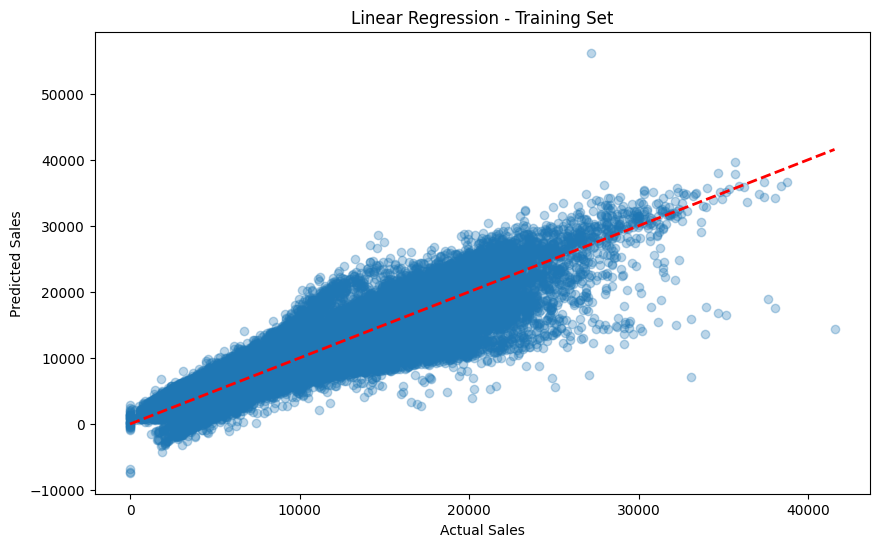
\includegraphics[width=0.9\textwidth]{Linear.png}
        \caption{Linear Regression}
        \label{linear} % Label for referencing the figure
    \end{minipage}\hfill
    \begin{minipage}{0.48\textwidth}
        \centering
        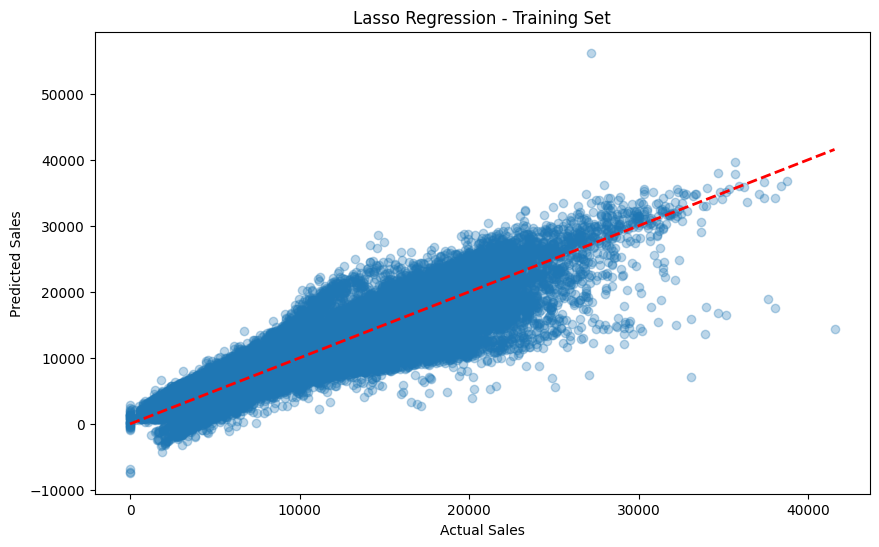
\includegraphics[width=0.9\textwidth]{lasso.png}
        \caption{Lasso Regression}
        \label{lasso} % Label for referencing the figure
    \end{minipage}

    % Second row with one image centered
    \vspace{0.5cm} % Adds vertical space between rows
    \begin{minipage}{0.6\textwidth}
        \centering
        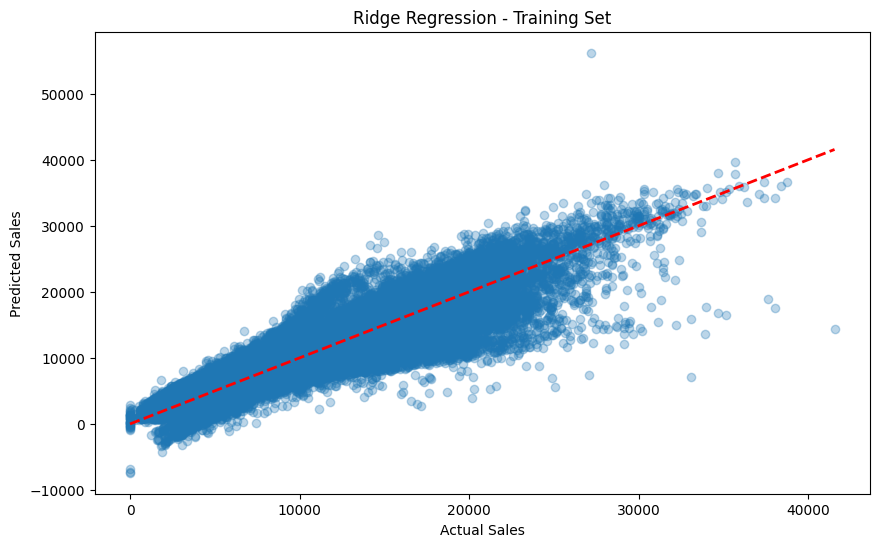
\includegraphics[width=0.9\textwidth]{ridge.png}
        \caption{Ridge Regression}
        \label{ridge} % Label for referencing the figure
    \end{minipage}
    
 
\end{figure}

High RMSE and MSE value and lower R-squared mean that regression models need more adjustment to have better performance. This model is not efficient enough to capture complexities and relationships in the data. The feature selection and feature scaling we implemented can be adjusted to improve the results. In addition, cross-validation and hyperparameter tuning will also improve the learning and prediction performance of the model.


\section{Decision Tree Regressor}

Decision Tree Regressor is a powerful machine learning algorithm used for regression tasks. It constructs a tree-like structure by recursively partitioning the feature space, making predictions based on the average value of the target variable within each region.

\subsection{Algorithm}

\begin{itemize}
    \item Tree Construction:
The decision tree is built by recursively splitting the data based on informative features. Each internal node represents a decision based on a feature, and each leaf node contains the predicted value. The goal is to minimize the variance of the target variable within each leaf node.

    \item Splitting Criteria:
Decision trees use various criteria such as MSE and R-squared to determine the best feature and threshold for splitting and evaluate impurity reduction for each possible split:
Impurity Reduction = [Impurity before split]- [Impurity after split]

    \item Recursive Splitting:
At each internal node, the algorithm selects the feature and threshold that maximally reduces the chosen criterion. The process continues until a stopping condition (e.g., maximum depth, minimum samples per leaf) is met.
-Prediction:
To predict a new instance, traverse the tree from the root to a leaf node based on feature values. The predicted value is the average of the target values in that leaf node.

    \item Advantages
-Interpretability: 
We can easily understand how the model arrives at its predictions by following the path from the root to a leaf.
-Handling Mixed Data: 
Decision trees handle both numerical and categorical features without requiring extensive preprocessing.
    \item  Disadvantages
-Overfitting: 
Decision trees tend to overfit the training data, resulting in poor generalization to unseen examples. Pruning techniques can mitigate this issue.
-Sensitivity to Small Variations: 
Small changes in the data can lead to different splits, affecting the tree’s structure.


\end{itemize}


\subsection{Results}







For hyperparameter tuning, we employed a combination of plotting and random search techniques to optimize hyperparameters for our machine learning model. Below, I outline the steps we took and the results we obtained.


\begin{itemize}
    \item Exploring Hyperparameter Relationships
Initially, we visualized the relationships between hyperparameters and model performance. By plotting these relationships, we gained insights into how different hyperparameter values impact the model's effectiveness. Based on the graph, we identified a suitable range within which to conduct our random search.

\end{itemize}


\begin{figure}[h] % Using [H] to force placement exactly here
    \centering

    % First row with two images side by side
    \begin{minipage}{0.48\textwidth}
        \centering
        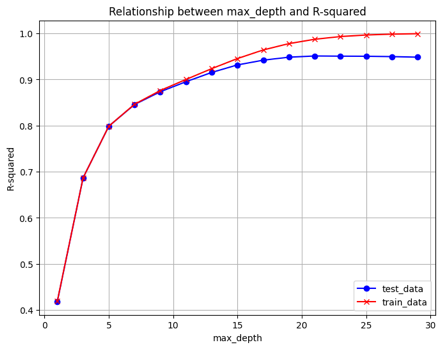
\includegraphics[width=0.9\textwidth]{unnamed.png}
        \caption{Max\_depth vs R\textsuperscript{2}}
        \label{pic1} % Label for referencing the figure
    \end{minipage}\hfill
    \begin{minipage}{0.48\textwidth}
        \centering
        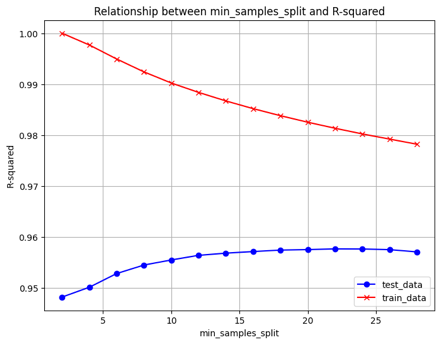
\includegraphics[width=0.9\textwidth]{unnamed-2.png}
        \caption{Min\_samples\_Split vs. R\textsuperscript{2}}
        \label{pic2} % Label for referencing the figure
    \end{minipage}

    % Second row with one image centered
    \vspace{0.5cm} % Adds vertical space between rows
    \begin{minipage}{0.6\textwidth}
        \centering
        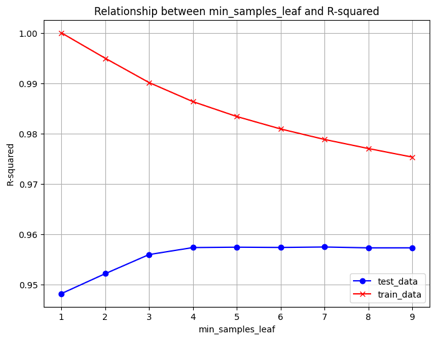
\includegraphics[width=0.9\textwidth]{unnamed-3.png}
        \caption{Min\_samples\_leaf vs R\textsuperscript{2}}
        \label{pic3} % Label for referencing the figure
    \end{minipage}
    
 
\end{figure}




% You can refer to the image using Figure \ref{fig:example-image}.


\begin{itemize}

    \item Random Search Ranges
For the hyperparameters, we set the following ranges:
- “max\_depth”: 15 to 25
- “min\_samples\_split": 15 to 25
- “min\_samples\_leaf”: 3 to 5
These ranges were chosen to strike a balance between model complexity and overfitting.

    \item Optimal Parameters
After performing random search, we discovered the optimal hyperparameters:
- “max\_depth”: 24
- “min\_samples\_leaf”: 4
- “min\_samples\_split”: 15
These values led to the best-performing model.

\end{itemize}

Since results of the train and test set suggest that there might be overfitting, we tried post pruning using ccp-alpha.
However no significant improvement was achieved.

\begin{table}[H] % Use [H] to force placement exactly here
    \centering
    \begin{minipage}{0.48\textwidth} % Adjust width as needed
        \centering
        \begin{tabular}{|l|c|c|}
            \hline
            \textbf{Metric} & \textbf{Training} & \textbf{Test} \\
            \hline
            R\(^2\) & 0.9801 & 0.9579 \\
            \hline
            MSE & 191540.02 & 403816.77 \\
            \hline
            RMSE & 437.65 & 635.47 \\
            \hline
        \end{tabular}
        \caption{Performance metrics for the Decision Tree Regressor with the best parameters found.}
        \label{tab:performance_metrics}
    \end{minipage}\hfill
    \begin{minipage}{0.48\textwidth} % Adjust width as needed
        \centering
        \begin{tabular}{|l|c|c|}
            \hline
            \textbf{Metric} & \textbf{Train} & \textbf{Test} \\
            \hline
            MSE & 191611.98 & 400628.78 \\
            \hline
            RMSE & 437.74 & 632.95 \\
            \hline
            R\(^2\) & 0.9801 & 0.9582 \\
            \hline
        \end{tabular}
        \caption{Performance metrics of the pruned model. Optimal alpha: 0.0421}
        \label{tab:pruned_model_metrics}
    \end{minipage}
\end{table}

Lastly, we benefitted Decision Tree Regressor to observe feature importance, with the results visible on figure \ref{fig:feature_image}. As expectedly, the most corralated factor appeared as the number of customers. 

\begin{figure}[H] % 'h' for placing the figure approximately here
    \centering
    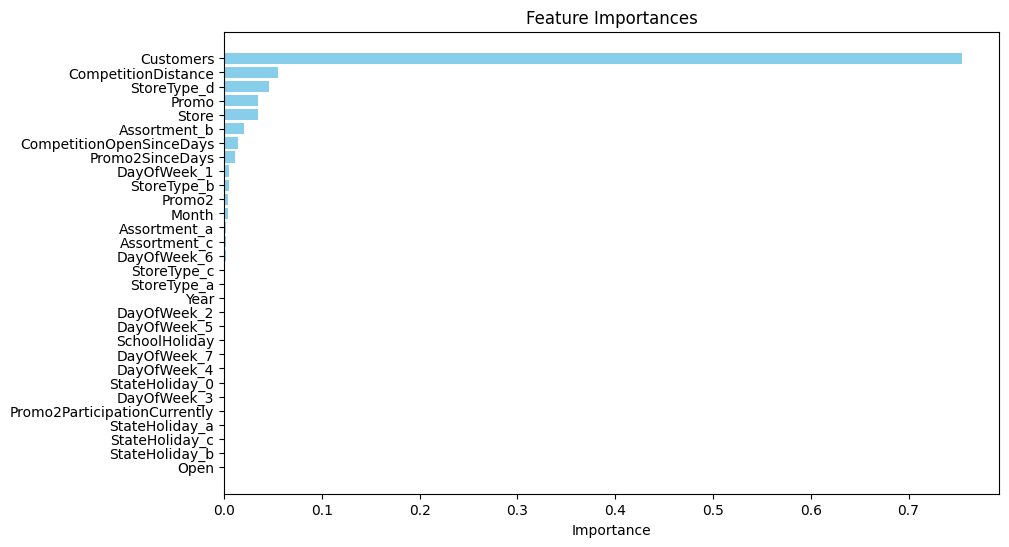
\includegraphics[width=0.8\textwidth]{feature.png} % Adjust width as needed
    \caption{Feature Importance according to DT Regressor} % Provide a caption
    \label{fig:feature_image} % Label for referencing the image
\end{figure}


\begin{figure}[H] % 'h' for placing the figure approximately here
    \centering
    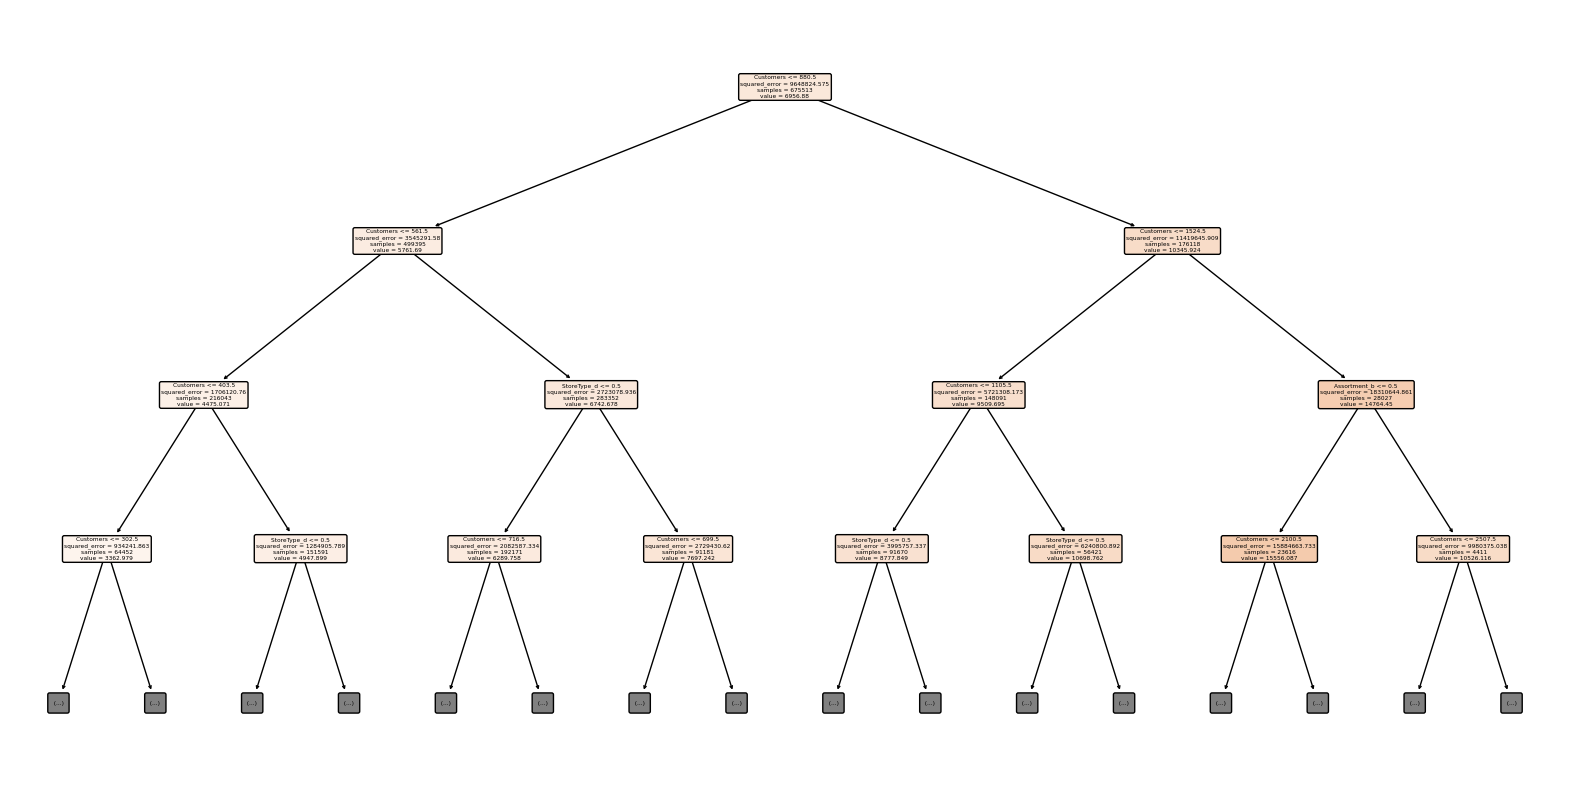
\includegraphics[width=0.8\textwidth]{dt.png} % Adjust width as needed
    \caption{First 3 layers of the DT Regressor} % Provide a caption
    \label{fig:dt} % Label for referencing the image
\end{figure}


\section{XGBoost (Extreme Gradient Boosting)}

XGBoost (Extreme Gradient Boosting) is a powerful implementation of the gradient boosting framework designed for efficiency and performance. It builds an ensemble of decision trees sequentially, each correcting the errors of the previous ones, to minimize a loss function (e.g., Mean Squared Error for regression or log loss for classification) combined with a regularization term to prevent overfitting. The objective function includes the loss function and a regularization term for model complexity, optimized using a greedy algorithm for node splits. Hyperparameter tuning involves adjusting parameters like learning rate, max\_depth, number of estimators, subsample, colsample\_bytree, and lambda, often using grid search or randomized search to enhance model performance. This approach helps in efficiently handling large datasets and achieving high predictive accuracy.

We initially did train-test-validation split on our train set. Then applied Standard scaling.
We did Hyperparameter Tuning using RandomizedSearchCV, furthermore the objective function for this task was set to mean squared error (MSE). 

Our model before hyperparameter tuning had RMSE OF 574.80 with R\_Squared 0.965. After applying the best parameters found through randomized search cv, we got the RMSE down to 432.58, with R\_Squared raised to 0.980.

\begin{table}[H] % Use [H] to force placement exactly here
    \centering
    \begin{tabular}{|l|c|c|}
        \hline
        \textbf{Model} & \textbf{RMSE} & \textbf{R\_Squared} \\
        \hline
        Before Hyperparameter Tuning & 574.80 & 0.965 \\
        \hline
        After Hyperparameter Tuning & 432.58 & 0.980 \\
        \hline
    \end{tabular}
    \caption{Performance metrics of the model before and after hyperparameter tuning.}
    \label{tab:model_performance}
\end{table}





\chapter{Results}
Table XX below summarizes the performance metrics (RMSE, R²) for the three models used in our project: Linear Regression, Decision Tree Regressor, and XGBoost.

\begin{table}[h]
    \centering
    \begin{tabular}{|l|c|c|p{5cm}|} 
        \hline
        \textbf{ } & \textbf{RMSE} & \textbf{R Squared (R2)}  \\
        \hline
        Linear Regression & 1238.84 & 0.840  \\
        \hline
        Decision Tree Regressor & 437.74 & 0.980 \\
        \hline
        XGBoost & 432.58 & 0.980 \\
        \hline
  
    \end{tabular}
    \caption{Comparison of the results}
\end{table}

Linear regression showed the highest RMSE value, indicating that the average error between the predicted and actual sales values is relatively high. The R² value of 0.23186 indicates that the model explains only about 84\% of the variance in the sales data. This suggests that the linear model is not capturing the underlying complexities and nonlinear relationships in the data effectively. The Decision Tree Regressor performed significantly better than the linear regression model. It achieved a much lower RMSE of 437.74. The R² value of 0.980 indicates that the model explains approximately 98\% of the variance in the sales data. This shows that the Decision Tree Regressor is highly effective at capturing the relationships in the data, leading to more accurate predictions. XGBoost outperformed the linear regression and performed slightly better than the decision tree regressor models. It achieved the lowest RMSE of 432.58, indicating the smallest average error between predicted and actual sales values. The R² value of 0.980 shows that XGBoost explains 98\% of the variance in the sales data, same as Decision Tree Regressor, demonstrating its ability to model complex relationships and provide accurate predictions.

In summary, the performance of the models improves significantly from linear regression to decision tree regressor, with XGBoost providing the best results as expected from a more advanced model. Linear regression, with the highest RMSE and lowest R², struggles to capture the complexities in the data. Decision Tree Regressor significantly reduces the prediction error and explains a high percentage of the variance. XGBoost further enhances the model performance, achieving the lowest prediction error and the highest R², making it the most effective model for this sales prediction task.




\chapter{Conclusion and Future Work}

For the term project, we evaluated the performance of Linear Regression, Decision Tree Regressor, and XGBoost models for predicting sales. XGBoost demonstrated the best performance with the lowest RMSE (432.58) and the highest R² (0.980), outperforming the other models. Incorporating more sophisticated techniques like ensemble methods or deep learning models could potentially enhance the predictive performance even further. Additionally, expanding the dataset to include more recent sales data and other external factors like economic indicators could provide deeper insights and more robust predictions.

\chapter*{References}

Dinçoğlu, P., \& Aygün, H. (2022, June). Comparison of Forecasting Algorithms on Retail Data. In 2022 10th International Symposium on Digital Forensics and Security (ISDFS) (pp. 1-4). IEEE.

Fattah J, Ezzine L, Aman Z, El Moussami H, Lachhab A. Forecasting of demand using ARIMA model. International Journal of Engineering Business Management. 2018;10. doi:10.1177/1847979018808673

Fildes, R., Ma, S., \& Kolassa, S. (2022). Retail forecasting: Research and practice. International Journal of Forecasting, 38(4), 1283-1318.

Kaushal, R. K., Giri, K. K., Kumar, H. S., Raina, K., Choudhury, D., \& Naikade, K. (2023, October). AI-Based Approach for Retail Sale Forecasting. In 2023 International Conference on Self Sustainable Artificial Intelligence Systems (ICSSAS) (pp. 111-116). IEEE.

Loh, W. Y. (2011). Classification and regression trees. Wiley interdisciplinary reviews: data mining and knowledge discovery, 1(1), 14-23.

Pedregosa, F., Varoquaux, G., Gramfort, A., Michel, V., Thirion, B., Grisel, O., Blondel, M., Prettenhofer, P., Weiss, R., Dubourg, V., Vanderplas, J., Passos, A., Cournapeau, D., Brucher, M., Perrot, M., \& Duchesnay, É. (2011). Scikit-learn: Machine Learning in Python. Journal of Machine Learning Research, 12, 2825-2830. Retrieved from https://scikit-learn.org/stable/documentation.html

Sajawal, M., Usman, S., Alshaikh, H. S., Hayat, A., \& Ashraf, M. U. (2022). A predictive analysis of retail sales forecasting using machine learning techniques. Lahore Garrison University Research Journal of Computer Science and Information Technology, 6(04), 33-45.

Seaman, B. (2018). Considerations of a retail forecasting practitioner. International Journal of Forecasting, 34(4), 822-829.

Zhang, G. P. (2005). Neural networks for retail sales forecasting. In Encyclopedia of Information Science and Technology, First Edition (pp. 2100-2104). IGI Global.


\end{document}
